In the second test, we prove the functionality of the algorithm in three dimensions. 

The algorithm compares the images and calculates the departure factor 
based on area of ROI. Fig. \ref{fig:target} demonstrates the 
tracking of $40$ images from initial position to the final position of the target, 
highlighted with red boxes;
the vector in blue describes the movement of the target. 

\begin{figure}[H]
\centering
  \subfloat[]{\label{fig:targeinit} 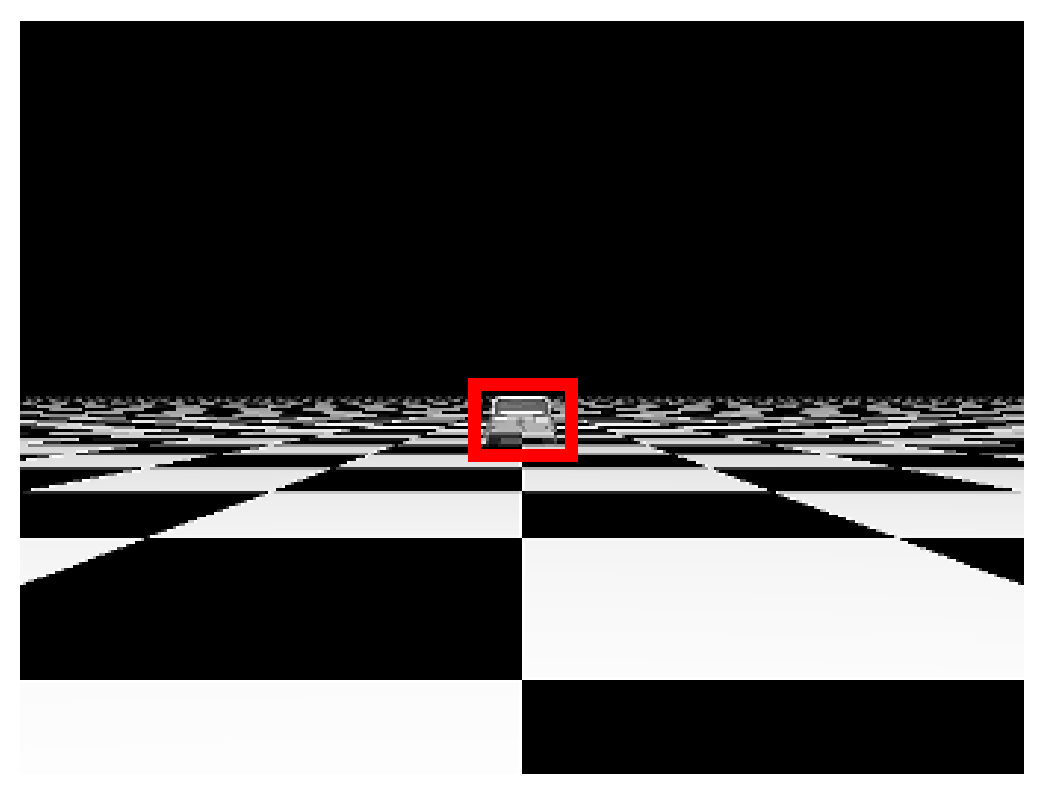
\includegraphics[width=.48\columnwidth]{images/figurea.eps}}
  \subfloat[]{\label{fig:targeend} 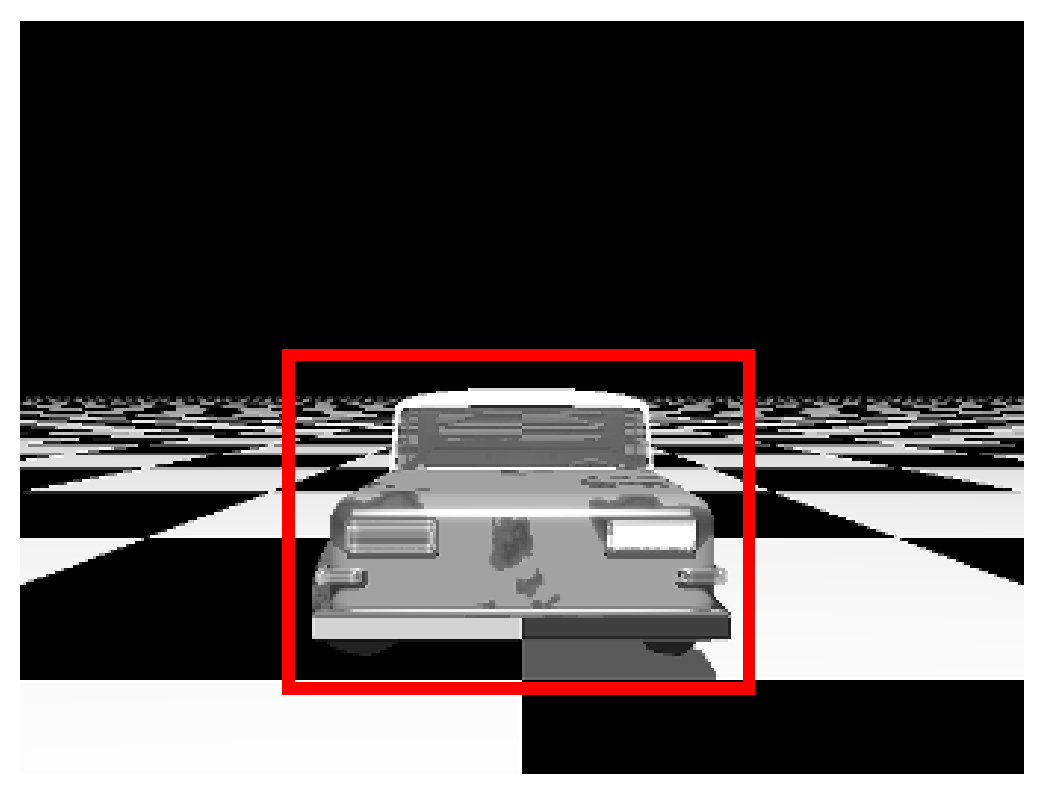
\includegraphics[width=.48\columnwidth]{images/figureb.eps}}
  \caption{The target in (a) is the initial position and its area is smaller than the target in (b), 
  which represents the final position. The factor is dividing both areas.}
  \label{fig:target}
\end{figure}

In Fig. \ref{fig:target}, we can observe an increase in ROI, and 
its influence to the departure factor is shown in Fig. \ref{fig:res_grapha_b}.

\begin{figure}[H]
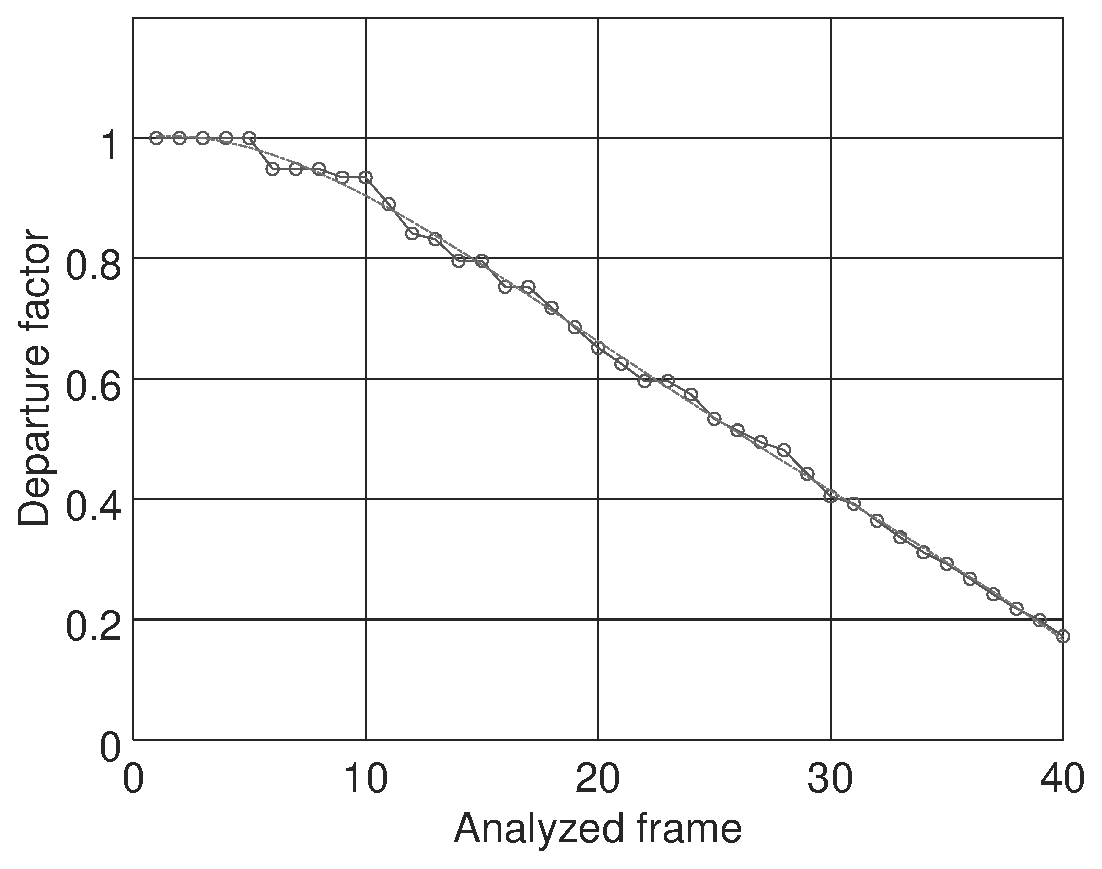
\includegraphics[width=\columnwidth]{images/grapha_b.eps}
\caption{Departure factor for each frame in the test 2.}
\label{fig:res_grapha_b}
\end{figure}

The Fig. \ref{fig:res_grapha_b} shows the departure factor in each frame
in test 2. If we interpret this value as the position in each sample time, 
then the departure factor describes the relative target position.
In the first image the analyzed target is at a distance $d_0$ 
and in the last image the target is at a distance of $17.18\%$ of $d_0$.
The departure distance decreases in discrete steps because the departure
factor is selected in discrete steps, if the target is
between two consecutive analysis layers (scales), the algorithm
approximates the target to the nearest layer.

\begin{figure}[!hbt]
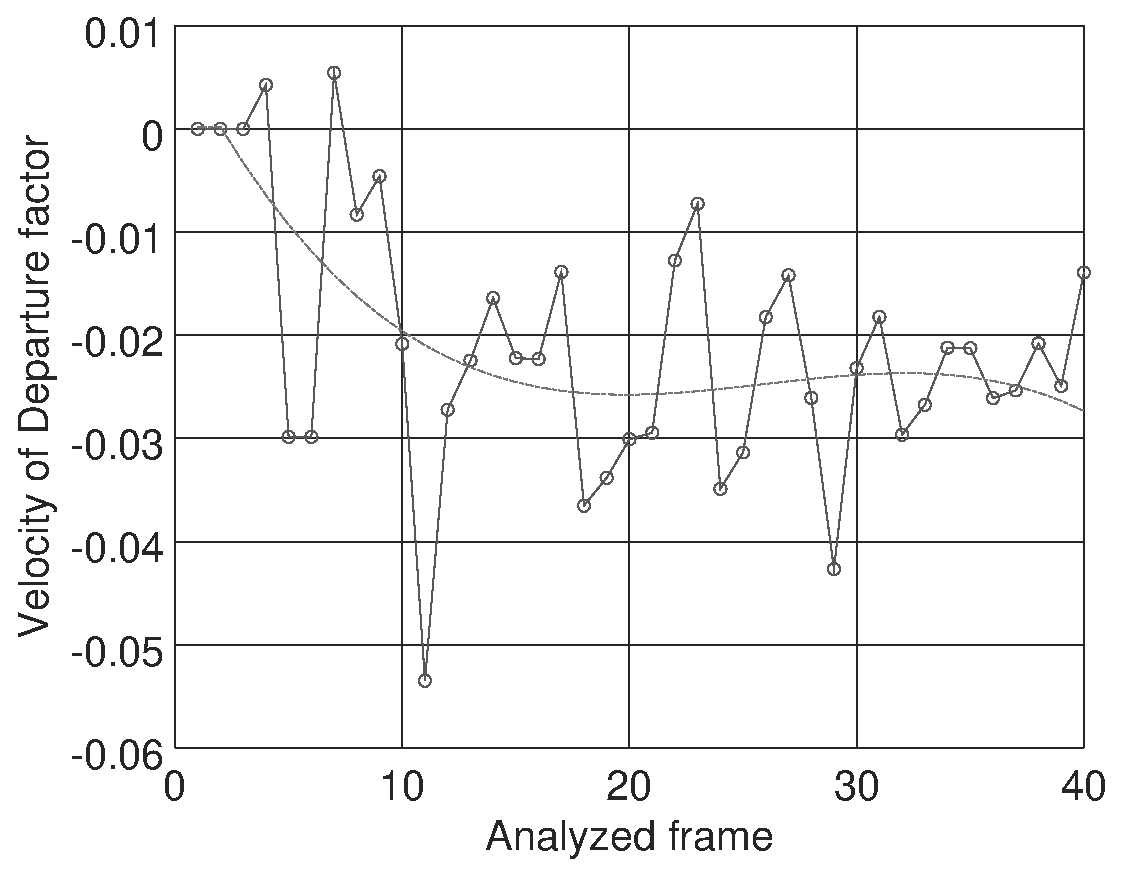
\includegraphics[width=\columnwidth]{images/graphvelocity.eps}
\caption{Velocity of departure factor for each frame in test 2.}
\label{fig:res_grapha_bv}
\end{figure}

Next table represents the bank of images used for test 2, totally 40 images generated by POV-Ray.
The frames are in the first column of table, second column are real distance between camera and target.
The proportion of real distances are in third column, it represents the approaching in percentage. For example, 
target in first frame is 23,5 meters from camera and considered 100\% of distance, in frame 40 the target is 04 meter 
from camera and 17,02\% in relation of first frame. Next column, fourth column, we have results of algorithm. 
Note in first frame, target is 100\% of distance and last frame 17,18\% of distance in relation of first frame.
Finally, last column is error between real proportion and proportion generated by algorithm. 
Error is diminishing when target is close (around 5 meters), it means algorithm has more precision 
when image of target is bigger because there are more information in ROI. It is a consequence of PCC, 
because in small ROI each pixel charge much information in comparative method. On other hands, if ROI is bigger,
the information is diluted around pixels. Then, algorithm has more date to compare.

\begin{table}[H]
\setlength{\tabcolsep}{1 pt} 
\caption{Table of comparative results}
\begin{tabular}{lllll}
Frames & Real Distances (m) & Proportion (\%) & Date of algorithm (\%) & Error (\%)\\
01 & 23,5 & 1 & 1 & 0 \\
10 & 18,5 & 78,72 & 93,46 & 15,77 \\
20 & 13,5 & 57,45 & 65,16 & 11,83 \\
30 & 8,5 & 36,17 & 40,46 & 10,60 \\
40 & 04 & 17,02 & 17,18 & 0,93
\end{tabular}
\end{table}

The velocity of departure factor is shown in 
Fig. \ref{fig:res_grapha_bv}, where the velocity is calculated
to $d_0=1$ and $\Delta t=1$. The value of the departure
velocities is negative, which indicates that the
target is approaching towards the observer. Relative velocity is calculated 
using the discrete-time derivate.
If we compare test 1 and 2 to the same $\Delta t=1$, it is evident 
that the departure velocity of  test 2  is lower than test 1. 
Note target approaches more in test 2 and, consequently, departure
velocity is lower than test 1.

